\section{Gumbo Nodes}
\label{section:gumbo_node}

In order to accurately profile the network, we have created minimum-cost hardware nodes to test the protocols on, which we have named
\textbf{GumboNodes}.  GumboNodes are barebones sensor nodes consisting of a microcontroller, a wireless transceiver, a sensor, and a battery. In our specific hardware, the system already comes on-board with a temperature sensor.  The goal of the network is to distribute updated sensor data to all the nodes in the network.

We selected the ATTiny85 as the microcontroller for the chip. The ATTiny85 is a low-cost, low-power 8-bit processor. It is Arduino-compatible and has a wide range of options to optimize the processor for power consumption. Table 1 provides power information from the datasheet [6]. In the lowest power mode, the processor uses less than 2 $\mu$A. There are only two ways to wake the chip from this deep sleep: an external interrupt caused by a logic level change on an input pin, or periodically by an internal oscillator known as the watchdog timer. The watchdog timer has maximum time limit of 8 seconds after which the microcontroller automatically wakes up and enters idle state. The system may immediately be put back to sleep, or act after it wakes up a certain number of times.

The Texas Instruments CC2500 was selected as the wireless chip. The CC2500 is a low-level 2.4GHz wireless transceiver. Communication occurs over a 4-wire serial perhiperal interface (SPI) [7]. The ATTiny85 we selected lacks an onboard SPI interface, but has a universal serial interface (USI) that is capable of interfacing with the transceiver. The CC2500 also has a temperature sensor on-board, which served as our sensor. 

%A flowchart of the node’s behavior is provided in Figure 1. After power-on, the system immediately goes into receive mode. If it does not hear a sync packet after a long enough period, the mote sends its own sync and 

\section{Proposed Protocols}

\subsection{Heart Beat Protocol}
\label{section:heart_beat_protocol}

\begin{figure}[h!]
  \centering
  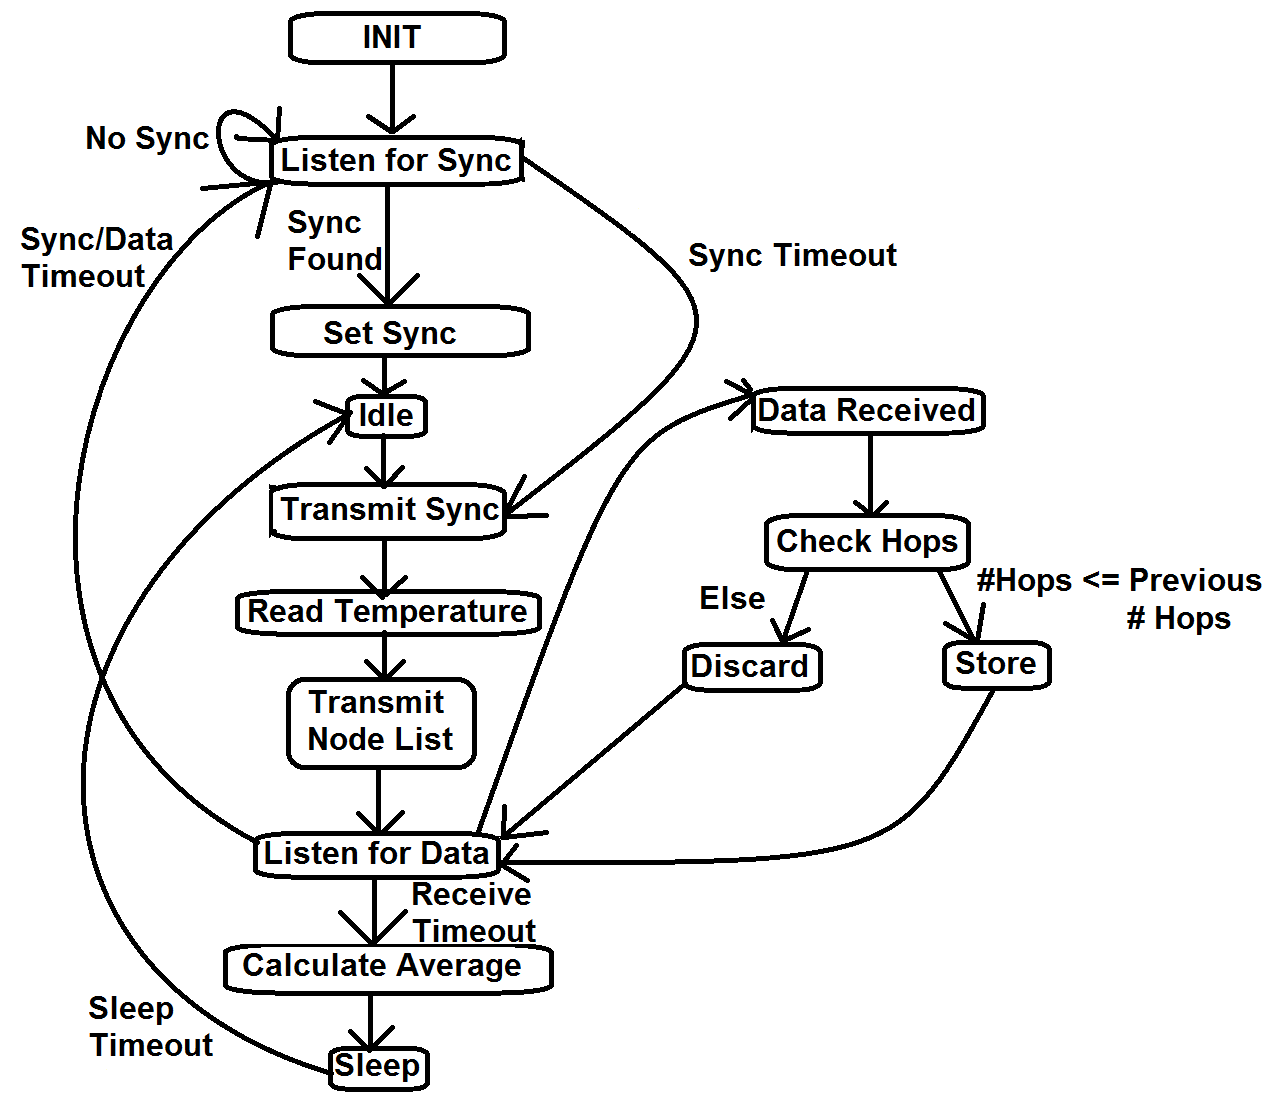
\includegraphics[width=0.5\textwidth]{images/algorithm_flowchart.png}
  \caption{A flowchart of the communication protocol
  \label{img:flowchart}
  }
\end{figure}

\begin{figure}[h!]
  \centering
  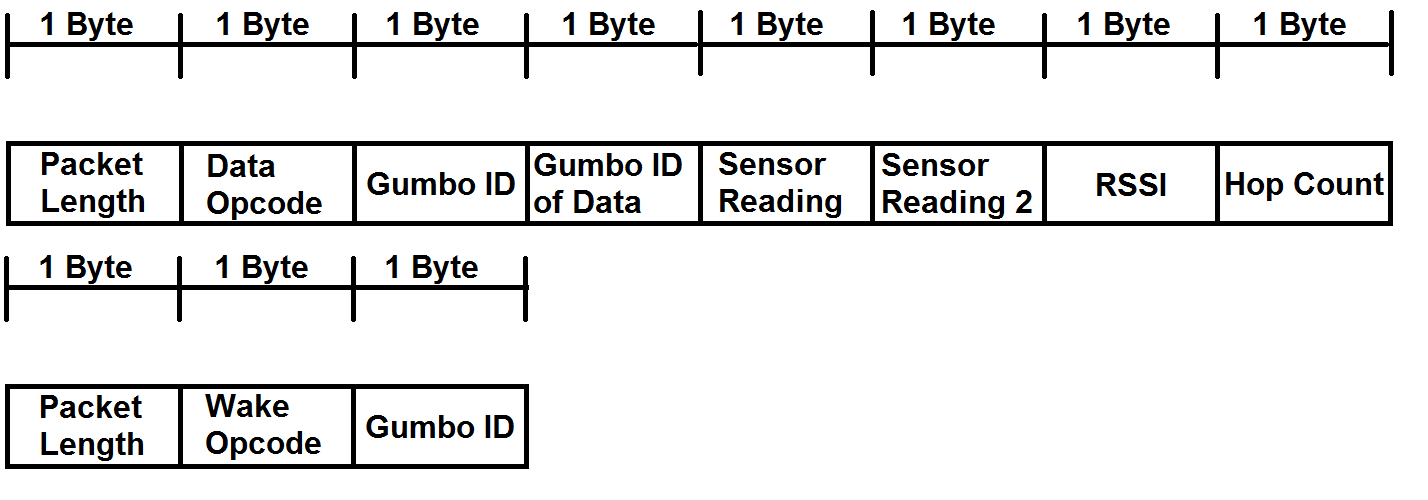
\includegraphics[width=0.5\textwidth]{images/data_packet.png}
  \caption{Data packet structure.
  \label{img:hb_packet}
  }
\end{figure}

Our first proposed solution was to dynamically sync nodes to an on-off pattern, a flowchart of the protocol is shown
in Figure~\ref{img:flowchart}.  The structure of a packet is shown in Figure~\ref{img:hb_packet}.  After power-on, the
system immediately goes into receive mode. If it does not hear a sync packet after a long enough period, the mote sends
its own sync and ............

\subsection{Random On/Off}
\label{section:random_dc}

\begin{figure}[h!]
  \centering
  \includegraphics[width=0.5\textwidth]{images/random_packet.png}
  \caption{Data packet structure used for the ``random'' communication protocol.
  \label{img:rand_packet}
  }
\end{figure}

We also wanted to explore the possibility of simply turning the radio on and off at random intervals, and syncing the
data when possible.  Though this is far less than ideal, it is significantly easier to implement, debug, and manage, and
a relatively low throughput rate may be acceptable for some applications.

In this protocol, the node wakes up and sends
a query packet asking for new data.  If another node responds to the request, it will send the data it stores, starting
with the most recently received.  If the data is new, it replaces any old reading and the receiver of the data sends a
packet asking for the next entry.  If the data is old, the receiver asks the sender to stop.  In order to determine the
``newer'' of two sets of data a simple counter is used, the node can account for the counter looping around by considering
a high number lower than a low number if the high number is close to the maximum possible value of the counter and the
low number is close to zero.  Although errors are possible with this system, its simplicity and redundancy may make it
favorable for some applications.  The results given in Section~\ref{section:evaluation}.
